%
%  Fast Sideways Composition, for COP 2016
%
% Confirmation Number:» 9
% Submission Passcode:» n/a
% MAX 6 PAGES
%
\RequirePackage[l2tabu, orthodox]{nag}
\PassOptionsToPackage{final}{graphics}
\documentclass[preprint,english,10pt,nonatbib]{sigplanconf}
\usepackage{myheader}
\addbibresource{references.bib}
\newacronym{api}{\textsc{api}}{application programming interface}
\newacronym{aop}{\textsc{aop}}{aspect-oriented programming}
\newacronym{cop}{\textsc{cop}}{context-oriented programming}
\newacronym{oop}{\textsc{oop}}{object-oriented programming}
\newacronym{oo}{\textsc{oo}}{object-oriented}
\newacronym{dsl}{\textsc{dsl}}{domain-specific language}
\newacronym{jit}{\textsc{jit}}{just-in-time}
\newacronym{vm}{\textsc{vm}}{virtual machine}
\newacronym{ffi}{\textsc{ffi}}{foreign-function interface}
\DeclareRobustCommand*\copa{\textsc{cop}\kern .12em\oldstylenums{09}\kern .12em a\xspace}
\DeclareRobustCommand*\copb{\textsc{cop}\kern .12em\oldstylenums{09}\kern .12em b\xspace}
\DeclareRobustCommand*\deltablue{\textsc{DeltaBlue}\xspace}

\begin{document}
\conferenceinfo{COP '16}{July 19, 2016, Rome, Italy}
\copyrightyear{2016}
\copyrightdata{978-1-nnnn-nnnn-n/16/07}
\copyrightdoi{nnnnnnn.nnnnnnn}

\publicationrights{licensed}     % this is the default

\titlebanner{DRAFT \--- not for distribution \--- DRAFT}        % These are ignored unless
\preprintfooter{Submitted to COP'16}

\title{Optimizing Sideways Composition}
\subtitle{Fast Context-oriented Programming in ContextPyPy}

% \authorinfo{Tobias Pape}
%            {Hasso Plattner Institute\\ University of Potsdam, Germany}
%            {tobias.pape@hpi.uni-potsdam.de}
% \authorinfo{Tim Felgentreff}
%            {Hasso Plattner Institute\\ University of Potsdam, Germany}
%            {tim.felgentreff@hpi.uni-potsdam.de}
% \authorinfo{Carl Friedrich Bolz}
%            {King's College, London}
%            {cfbolz@gmx.de}
\authorinfo{Tobias Pape\textsuperscript{*} \and Tim Felgentreff\textsuperscript{*\textdagger} \and Robert Hirschfeld\textsuperscript{*\textdagger}}
           {\textsuperscript{*}Hasso Plattner Institute, University of Potsdam, Germany\\
           \textsuperscript{\textdagger}Communications Design Group (CDG), SAP Labs, USA\\
           \textsuperscript{\textdagger}Viewpoints Research Institute, USA}
           {\{firstname\}.\{lastname\}@hpi.uni-potsdam.de}

\maketitle

\begin{abstract}
  The prevalent way of code sharing in many current object systems is static
  and/or single inheritance; both are limiting in situations that call for
  multi-dimension decomposition. Sideways composition provides a technique to
  reduce their limitations. \Ac{cop} notably applies sideways composition to
  achieve better modularity. However, most \ac{cop} implementations have a
  substantial performance overhead. This is partly because weaving and
  execution of layered methods violate assumptions that common language
  implementations hold about lookup. Meta-tracing \ac{jit} compilers have
  unique characteristics that can alleviate the performance overhead, as they
  can treat lookup differently.

  We show that meta-tracing \ac{jit} compilers are good at optimizing
  sideways composition and give initial, supporting results. Furthermore, we
  suggest that explicit communication with the \ac{jit} compiler in a \ac{cop}
  implementation can improve performance further.
  \end{abstract}

\category{D.3.3}{Programming Languages}{Language Constructs and Features}
\category{D.3.2}{Programming Languages}{Language Classifications}[Mul\-ti\-par\-a\-digm languages]
\category{D.3.4}{Programming Languages}{Processors}[Run-time environments]

\keywords
context-oriented programming,
meta-tracing \acs{jit} compilers,
optimization,
virtual machines,
PyPy

\section{Introduction}



% \paragraph*{Contributions}

In this work, we make the following contributions and show
\begin{itemize}
\item that the performance overhead of sideways composition is still
  present in most \ac{cop} implementations;
\item that meta-tracing--based \ac{jit} compilation can reduce the
  overhead of sideways composition; and
\item that communicating the active layer composition \emph{explicitly} to the
  \ac{jit} compiler can further reduce the overhead of sideways composition.
\end{itemize}


\section{\protect\Acs{cop} and Meta-tracing \acs{jit} Compilers}

We briefly describe the performance impact of \ac{cop} implementations and
introduce meta-tracing \ac{jit} compilers.

\subsection{The Performance of \acs{cop}}
\label{sec:performance-cop}
\ac{cop} as a modularity mechanism to dynamically adapt behavior at run-time has
been demonstrated to be useful in a variety of scenarios. Beyond its original
motivation for dynamically adapting systems based on environmental factors such
as battery level, geolocation, or time of day~\todo{cite}, \ac{cop} has also
been applied to provide safety in the development of live
systems~\cite{lincke+:2012:scoping-changes} or to let multiple conflicting
versions of programming interfaces co-exist~\todo{cite my talk cop 2013}.

% ~\cite{lincke+:2011:implementing-scoped}

However, as with many abstraction mechanisms, \ac{cop} comes with some overhead,
a fact that has been repeatedly recognized. Context layer aware method lookup
requires additional operations at run-time. Most \ac{cop} extensions to dynamic
languages use the host languages meta-programming facilities to redirect method
dispatch, whereas statically compiled languages require additional compilation
steps to construct data structures to track layer activation states at
run-time. Both of these solutions come with considerable performance decrease
from \SIrange{75}{99}{\percent}~\cite{appeltauer+:2009:comparison-context-oriented}.


\subsection{Meta-tracing Just-In-\kern-0.12emTime Compilers}
\label{sec:meta-tracing-jit}

\Acf{jit} compilation is one of the most used technique for speeding up the
execution of programs at run-time. Many language implementations have yet
benefitted from \ac{jit} compilers, including but not limited to today's
popular languages such as Java~\cite{paleczny+:2001:java-hotspot} or
JavaScript~\cite{holtta:2013:crankshafting-from}. A particular implementation
approach for \ac{jit} compilers is to us \emph{tracing}, that is, recoding the
steps an interpreter takes to obtain its instruction sequence, a \emph{trace}.
This trace is subsequently used instead of the interpreter to execute the same
part of that program~\cite{mitchell:1970:design-construction} at higher speed.
Native code~\cite{bala+:2000:dynamo:-transparent} as well as object-oriented
programs~\cite{gal+:2006:hotpathvm:-effective} have already been optimized
using this technique.

With \emph{meta-tracing} the execution of the interpreter is observed instead
of the execution of the application program. The resulting traces are therefore
not specific to the particular application but to the underlying
interpreter~\cite{bolz+:2009:tracing-meta-level:}. This way, language
implementers do not have to implement optimized language-specific \ac{jit}
compilers but rather to provide a straightforward language-specific interpreter
that is subject to the meta-tracing technique. \emph{Hints} enable
communication with and hence fine-tuning of \ac{jit}
compiler~\cite{bolz_runtime_2011}.

\section{Faster Sideways Composition with Meta-tracing}

We propose that meta-tracing \ac{jit} compilers can reduce the overhead of
sideways composition and \ac{cop}, and that \emph{promoting} the composition of
active layers can reduce the overhead even further.

\subsection{Employing a Meta-tracing \protect\acs{jit}}
\Acl{cop} employs sideways composition to inject context-dependent behavioral
changes into an existing hierarchy of behavior. These hierarchies are typically
defined by the static and/or single inheritance of object systems. These
hierarchies are typically important for execution time performance, as they
form the basis for \emph{lookup}.

Most execution environments, such as \acp{vm} for dynamic object-oriented
languages, assume that those hierarchies change rarely and hence lookup can be
fast. However, using sideways composition to alter behavior invalidates this
assumption. Especially, since \ac{cop} explicitly redefines lookup based on
currently active layers; the composition of currently active layers becomes
\emph{crucial} for calculating the lookup in the dynamic extent of executed
code. If this composition stays the same, lookup stays the same, if it changes,
lookup may change. Execution environments typically have to decide, whether to
always re-exercise the lookup for every method under the active layers, or
cache (and invalidate) lookup information when the composition of active layers
changes. For example in the sequence
\begin{lstlisting}
-- active layers: §\(\emptyset\)§
method1()
  activate(layer1)
    method2()
  deactivate(layer1)
\end{lstlisting}
a \ac{cop} implementation typically uses one of the following two strategies:
\begin{enumerate}
\item lookup \lstinline|method1()| under the composition
  \(\emptyset\)
  and lookup \lstinline|method2()| under the composition
  [\lstinline|layer1|], or
\item use cached lookup information for \lstinline|method1()|, switch cached
  lookup information due to change in active layers, use (new) cached lookup
  information for \lstinline|method2()|.
\end{enumerate}
Both cases effect a performance impact either on every lookup or on every
layer change.

With meta-tracing \ac{jit} compilers, however, this effect is much less
severe. Although rarely-changing lookup still is helpful for its operation, a
change in lookup \--- for example induced by a layer activation \--- can be
anticipated and be accounted for.

Thus, with a properly instructed meta-tracing \ac{jit} compiler, a third option
becomes available. At points in the execution where the composition of active
layers becomes important, a \emph{guard} ensures that this composition did not
change. While counter-intuitive at first, this actually is a benefit. When a
certain different composition has been encountered often enough at the guard,
the meta-tracing \ac{jit} compiler will introduce a \emph{bridge} into a new
part of a trace, in which \emph{this} different composition can be assumed not
to change, and lookup can be optimized accordingly. Note that this resembles
strategy 2 above, but is implicit and actually guided by the \ac{jit} compiler.
Therefore, the actual \ac{cop} implementation does not have to manage the
caching information when altering the lookup information, saving both execution
time and implementation complexity.

\subsection{Promoting the Compositions of Active Layers}

The compositions of active layers is crucially important for the lookup in
\ac{cop}, and all strategies above reflect this. However, only the
language-level implementation of \ac{cop} actually knows about the
composition's importance, and even for meta-tracing \ac{jit} compiler's
strategy, the \ac{jit} compiler first hast to become aware of the fact that the
composition is \--- indeed \--- important for its trace. Yet, the \ac{jit}
compile can only apply heuristics to identify the composition as
trace-important.

This situation is commonly known when implementing \acp{vm} that use a
meta-tracing \ac{jit} compiler. Based on the value of a certain object it may
be desirable to \emph{specialize} traces to these values (essentially what
happened above with the guard and the bridge).
Implementers can chose to \emph{promote}~\cite[\S
3.1]{bolz+:2011:runtime-feedback} such an object and the \ac{jit} compiler will
ensure that traces are actually specialized to the object's values,  regardless
of wether the \ac{jit} compiler's \emph{heuristics} would result in the same
specialization or not. If applied carefully, this promotion can decrease
execution time.

Up until recently, this \emph{promotion} of objects had not been available to
language-level implementers of \ac{cop}. However, at the time of writing, one
\ac{vm} with meta-tracing \ac{jit} compiler (PyPy) exposes the \emph{promote}
functionality to the language-level and it is possible to use it for a \ac{cop}
implementation. The composition of active layers can now be promoted and the
meta-tracing \ac{jit} compiler now ensures that (a) a specialized traces exists
for each encountered composition, and (b) within a given trace, the composition
wont change and can be relied upon. This assumption now can be made when
exercising lookup during execution, saving execution time.


\section{<<Impl: ContextPy, VM interface, applevel promote>>}


%
\section{Performance Evaluation with \acs{cop}}

\begin{figure*}
  \centering
  \hbox to \linewidth{\hss
  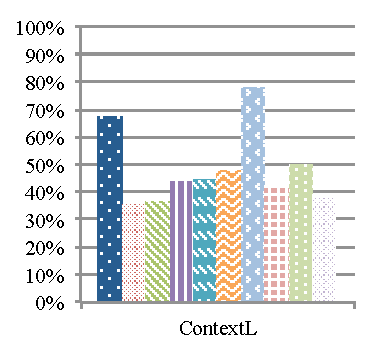
\includegraphics[height=6\baselineskip]{bench/malte-a/malte-a-3}
  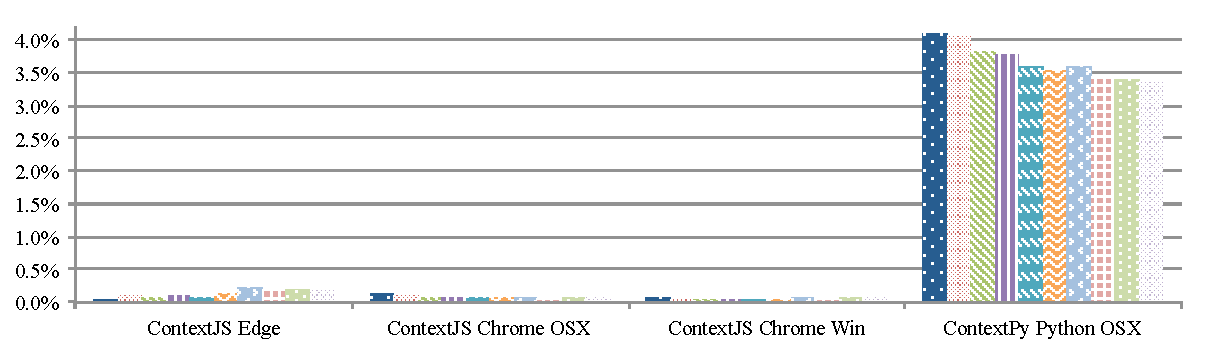
\includegraphics[height=6\baselineskip]{bench/malte-a/malte-a-2}
  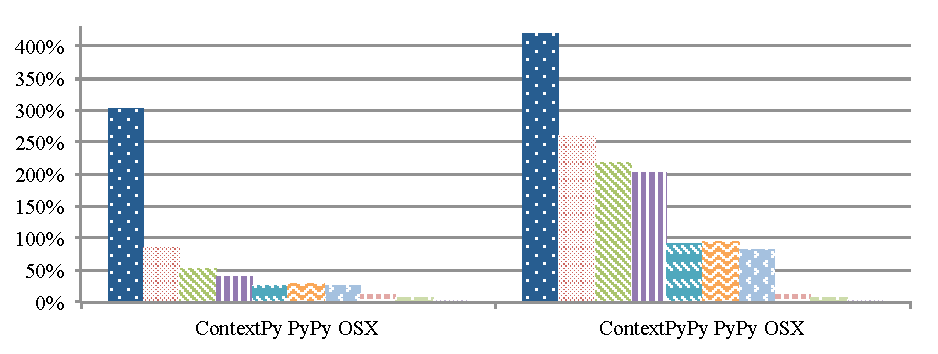
\includegraphics[height=6\baselineskip]{bench/malte-a/malte-a-4}
  \hss}
\caption{Results of \copa. Relative throughput of method execution in
  \protect\acs{cop} implementations with (each left to right) 0 to 10 layers
  normalized to the respective non-layered workload. Higher is better. For raw
  numbers see \autoref{tab:copa} and \autoref{tab:copall}. (Note
  the different scales, see \autoref{fig:malte-a-overview} for an overview
  comparison.)}
  \label{fig:malte-a}
\end{figure*}



As described in the introduction, we evaluate the following:
\begin{enumerate}
\item Sideways composition \emph{still} has a considerable impact on execution
  time.
\label{item:1}
\item Meta-tracing \ac{jit} compilers can alleviate the performance impact of
  sideways composition on execution time.
\label{item:2}
\item Explicit \emph{promotion} of the active layer composition can further
  improve execution time.
\label{item:3}
\end{enumerate}
%
For \ref{item:1}, we re-run in parts benchmarks presented in
2009~\cite{appeltauer+:2009:comparison-context-oriented}, which showed a
performance impact of sideways composition as used with \ac{cop}
implementations. For \ref{item:2}, we additionally augment the well-known
DeltaBlue benchmark~\cite{freeman-benson+:1989:deltablue-algorithm:} with
layers and additional functionality and compare the impact of sideways
composition on platforms with and without meta-tracing \ac{jit} compilers.
For \ref{item:3}, we run both benchmarks with a \emph{promote}-enhanced
\ac{cop} implementation, as well.
We present and discuss the most important results for each benchmark and
provide all results in the appendix.

\subsection{Setup}
\label{sec:setup}


\paragraph{System} We executed the benchmarks on %
% MacBook Pro Tobi
an Intel Core i7-4850HQ at \SI{2.3}{\GHz} with \SI{6}{\mega\byte} cache and
\SI{16}{\giga\byte} of RAM. The machine ran Mac OS\,X 10.9.5.
%%%% Surface Tim??
Certain benchmarks were run on an Intel Core i7-4650U at \SI{1.7}{\GHz} with
\SI{4}{\mega\byte} cache and \SI{8}{\giga\byte} of RAM, this machine ran
Windows 10.
%
%%%% Maxinchen
% an Intel Xeon E5-2650 (Sandy Bridge)  at \SI{2.8}{\GHz} with
% \SI{20}{\mega\byte} cache and \SI{16}{\giga\byte} of RAM. 
% Although virtualized on Xen, the machine was idle.
% The machine ran Ubuntu 14.04.1 LTS with a \SI{64}{\bit} Linux 3.2.0.

\paragraph{Implementations} %

We used ContextPy\footnote{{\smaller\url{https://bitbucket.org/cfbolz/contextpy/}}
  rev 5155cb7.} with Python 2.7.5 and PyPy 5.1 on OS\,X and
ContextPyPy\footnote{ContextPy as above but with explicit \emph{promote}.} with
PyPy 5.1 on OS\,X in both benchmarks. Additionally, for the re-run of the 2009
benchmark, we used
ContextJS~\cite{lincke+:2011:open-implementation}\footnote{{\smaller\url{https://github.com/LivelyKernel/LivelyKernel/tree/master/core/cop}}
  rev 0bd117c.} with V8 (Chrome 50.0.2661.66 beta 64-bit) on OS\,X, Chakra
(Edge 25.10586) on Windows 10 and V8 (Chrome 49.0.2623.112) on Windows 10; as
well as LispWorks\textsuperscript{\textregistered} 64-bit 7.0.0 on OS\,X.

Introducing layers with ContextPy increases the initial size of the traces
beyond PyPy's standard maximum trace limit. Therefore, we use a slightly
altered build of PyPy 5.1 that allows a much higher trace limit than the
standard build.


\paragraph{Methodology} 
% INITSIZE = 200000
% MAXSIZE = 1000000000
% TARGETTIME = 5.0 * 1000
For \copa and \copb (see \autoref{sec:benchmarks}), every benchmark was run with increasing size until a
measurement took at least 5 seconds; this matches the original
methodology~\cite{appeltauer+:2009:comparison-context-oriented}. Warm-up is
provided by the not measured runs. 
% ITER_DEFAULT=${ITER:-5}
% SIZE_DEFAULT=${SITE:-18000}
% WARM_DEFAULT=${WARM:-3}
For \deltablue (see \autoref{sec:benchmarks}), every benchmark was run 5 times
uninterrupted in a new process with additional 3 times warm-up prior to
measurement for PyPy\footnote{Python did not exhibit any warm-up--related
  differences/}. The execution time was always measured \emph{in-system} and,
hence, does not include start-up. We show the arithmetic mean of all runs along
with bootstrapped~\cite{davison+:1997:confidence-intervals} confidence
intervals for a \SI{95}{\percent} confidence level.

%\footnote{Raw figures can be  found as an appendix (\autoref{tab:all})}

% \paragraph{Availability}  All of our benchmarks and infrastructure
%  are available at <<TBD>>.


\subsection{Benchmarks}
\label{sec:benchmarks}

Our first set of benchmarks is taken from one of our earlier
papers~\cite{appeltauer+:2009:comparison-context-oriented}. These
micro-benchmarks attempt to measure the pure performance overhead of
dispatching to active layers and of layer activation. In the first part of
these benchmarks (\copa), we use an object with ten integer variables
(\texttt{counter\textsubscript{1}} to \texttt{counter\textsubscript{10}}) that
provides ten methods (\texttt{method\textsubscript{1}} to
\texttt{method\textsubscript{10}}), where each \texttt{method\textsubscript{i}}
increments all counters from \texttt{counter\textsubscript{1}} to
\texttt{counter\textsubscript{i}} by one. The same behavior is provided by a
method \texttt{layered}. The base method increments only
\texttt{counter\textsubscript{1}}, and nine layers
(\texttt{Layer\textsubscript{1}} to \texttt{Layer\textsubscript{9}}) provide a
partial method to adapt the base method to each increment one of the other
counters. Running just the \texttt{layered} method without any layers being
active thus yields the same behavior as \texttt{method\textsubscript{1}}.


In the second part (\copb) of our first benchmark set, we measure the
performance impact of layer activation. For most \ac{cop} languages, layer
activation means updating internal data structures with the current layer
composition. To quantify this impact, we measured the execution time of running
five methods (\texttt{method\textsubscript{1}} to
\texttt{method\textsubscript{5}}) in succession that each increment one
counter. We compare this to the execution time of five partial methods from
five layers that implement the same method body, where each layer is activated
in succession.


\def\idBox#1#2{%
\setlength{\fboxsep}{1pt}%
% \colorbox[HTML]{#1}{\textcolor[gray]{0.9}{\rule[0.1pt]{0pt}{5pt}#2}}%
\colorbox{#1}{\textcolor[gray]{0.9}{\rule[0.1pt]{0pt}{5pt}#2}}%
\xspace}
% DeltaBlue~\idBox{blue}{\(\circ\)}, %
% DeltaPurple ~\idBox{purple}{\(\bigtriangleup\)}, %
% DeltaViolet ~\idBox{violet}{\(\square\)}, %
% DeltaRed~\idBox{red}{\(+\)}, %
%  % ~\idBox{}{\(\boxtimes\)}, %
%  % ~\idBox{E41A1C}{\(\)}, %

Our second benchmark (\deltablue) measures the relative overhead of sideways
composition on a more wide-spread benchmark, DeltaBlue. For that, we augmented
DeltaBlue with additional functionality (reversed lists for storage, count of
constraint executions and binary constraints), both statically added to the
benchmark (Delta\emph{Purple}~\idBox{purple}{\(\bigtriangleup\)})
and dynamically composed via layers (Delta\emph{Red}~\idBox{red}{\(+\)}).
To measure the overhead of the mere presence of dynamic sideways composition
functionality without actually using it, we also measured DeltaRed with all
layers deactivated (Delta\emph{Violet} ~\idBox{violet}{\(\square\)}).
We normalize the execution time of all four benchmarks to
Delta\emph{Blue}~\idBox{blue}{\(\circ\)}
on each implementation and \ac{vm}. That way, we show the overhead of the
\ac{cop} implementation rather than mere execution time.

% All benchmarks are single-threaded.

\subsection{Results}

\begin{figure*}
  \centering
  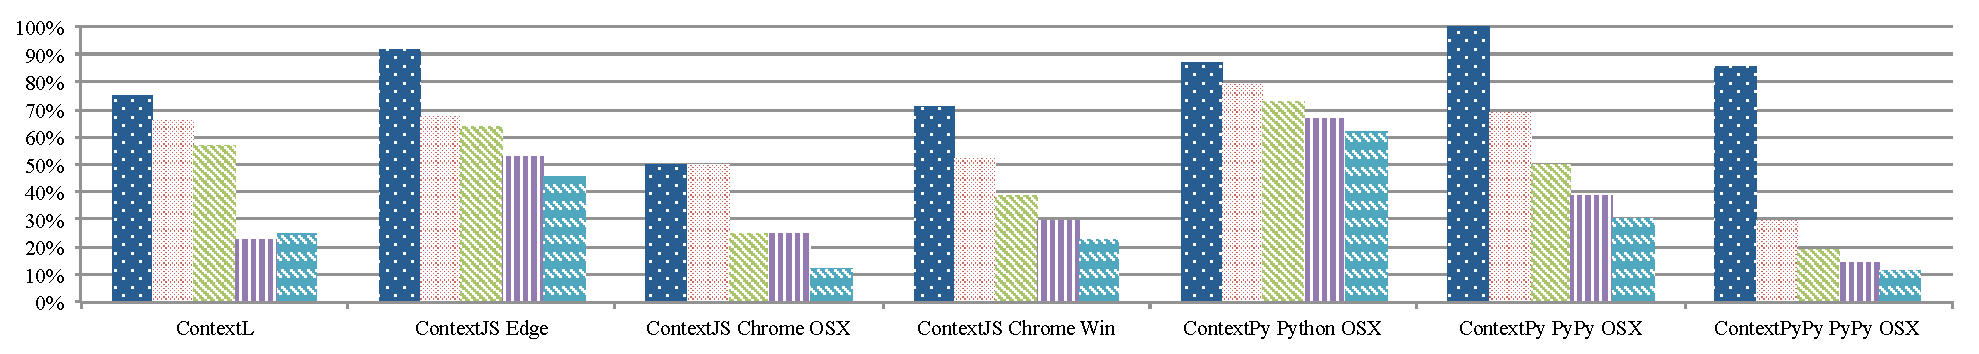
\includegraphics[width=.85\linewidth]{bench/malte-b}
  \caption{Results of \copb. Relative throughput of layer activation in
    \protect\acs{cop} implementations with (each left to right) 1 to 5 layers
    normalized to a workload with no layers active whatsoever. Higher is
    better. For raw numbers see \autoref{tab:copb} and \autoref{tab:copall}.}
  \label{fig:malte-b}
\end{figure*}

The results of the \copa benchmark are shown in \autoref{fig:malte-a}. We
evaluated the performance by comparing each ordinary method
\texttt{method\textsubscript{i}} with the execution performance of activating
all layers from \texttt{Layer\textsubscript{1}} to
\texttt{Layer\textsubscript{i}} (which gives the same behavior) and normalizing
to the ordinary method. As we reported in our previous work, ContextL shows a
performance degradation ranging from \SIrange{22}{65}{\percent}. Interestingly,
the decrease in performance does not seem to correspond to the number of active
layers, likely due to the variability of the optimizations of the underlying
Lisp \ac{vm}. On the V8 and Chakra JavaScript \acp{vm}, ContextJS incurs a
massive performance hit of over \SI{99.7}{\percent} in all cases, even where no
layer is active. ContextPy on the Python \ac{vm} is little better with overhead
around \SI{95}{\percent}.

Running ContextPy on PyPy, that is, using a meta-tracing \ac{jit} compiler,
yields vastly different results. Against the trend of the other
implementation/platform combinations, using \ac{cop} layers can actually
\emph{increase} performance. When just layers are present but not activated,
ContextPy on PyPy can gain a \(3.5\times\) speedup and ContextPyPy even over
\(4\times\). Compared with ContextPy on Python, the relative performance
difference is up to two orders of magnitude improved.

Moreover, ContextPyPy manages to retain a speedup of at least \(2\times\)
over the non-layered version up to three active layers, exhibiting only minor
slowdown for four to six active layers. After that, the performance levels up
with ContextPy on PyPy. We attribute the latter, rather steep decline in
performance to how the meta-tracing \ac{jit} compiler handles rather long
traces that can occur with an increasing number of active layers and which are
yet to be investigated.

\paragraph{Discussion} The meta-tracing \ac{jit} compiler of PyPy appears to be
effective at eliminating the overhead of sideways composition. The results of
ContextPyPy suggest that communicating layer information properly can vastly
improve this effect, too.
%

\medskip\noindent %
The results of the \copb benchmark are shown in \autoref{fig:malte-b}. The
performance impact for layer activation for each of the tested systems is
comparable and clearly increases as more layers are activated. Moreover,
ContextPy on Python \--- the only implementation/platform combination without
\ac{jit} or \ac{jit}-like optimizations \--- exhibits the least severe impact
with increasing layers.

\paragraph{Discussion} The meta-tracing \ac{jit} compiler of PyPy seems to have
to invalidate assumptions on layer activations, possibly not being able to
re-use certain traces. The results of ContextPyPy suggest that the current way
of communicating layer information to the meta-tracing \ac{jit} compiler in
fact can also hamper optimizations, that is, such \emph{hints} have to
be used with great care.

\begin{figure*}
  \centering
  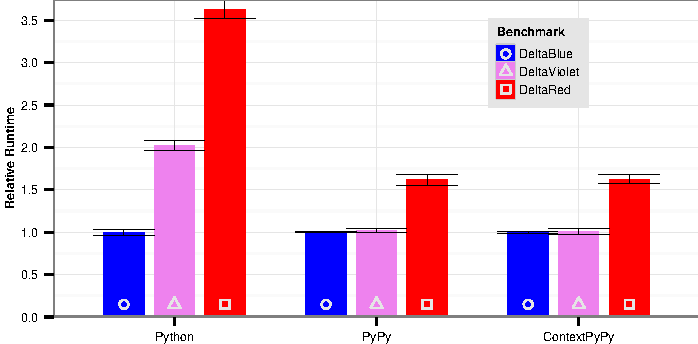
\includegraphics[width=.55\linewidth]{bench/DeltaBlue-norm.pdf}
  % 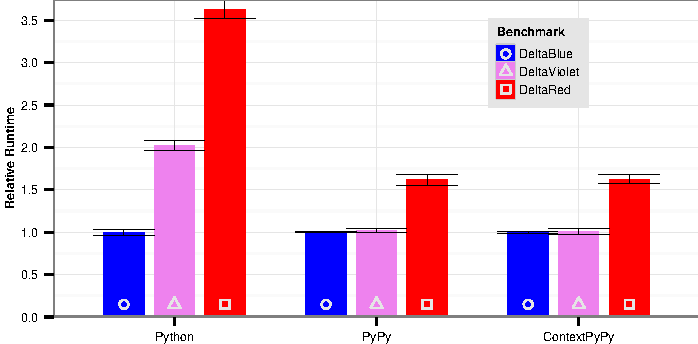
\includegraphics[width=.48\linewidth]{bench/DeltaBlue-norm.pdf}
  % \hfil
  % 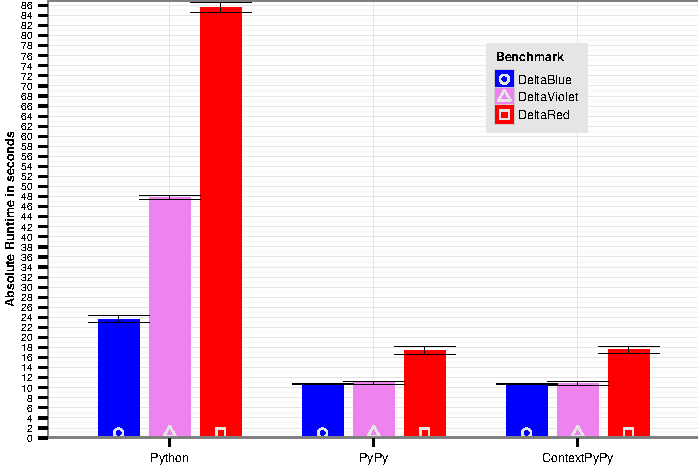
\includegraphics[width=.48\linewidth]{bench/DeltaBlue.pdf}
  \caption{Results of \deltablue. Relative execution time of Delta\ldots benchmarks
    on ContextPy on Python and PyPy; and ContextPyPy. Normalized to DeltaBlue.
    Lower is better. For raw numbers see \autoref{tab:deltablue-raw}.}
  \label{fig:deltablue}
\end{figure*}

\medskip\noindent %
The results of the \deltablue benchmark are shown in \autoref{fig:deltablue}.
Expectedly, the additional workload of DeltaPurple over DeltaBlue is comparable
across all three implementation/platform combinations. However, the mere
presence of layered methods (DeltaViolet) has a comparatively high impact on
Python, with up to \(3\times\)
slowdown. At the same time, virtually no overhead is present on PyPy for
DeltaViolet. The overhead of activated layers (DeltaRed) is quite severe on
Python, ranging about \(5\times\)
of DeltaPurple, whereas on PyPy the slowdown is less than \SI{50}{\percent}
(\(\approx 1.4\times\)). ContextPyPy performs virtually the same as ContextPy
on PyPy.

\paragraph{Discussion} \deltablue, being a less ``micro'' benchmark, reinforces
the impression of \copa than the meta-tracing \ac{jit} compiler of PyPy is
effective at eliminating the overhead of sideways composition. Especially the
no-layers-activated case having no overhead seems important for wider adoption.
Seeing \copa and \copb, the indifference between ContextPy on PyPy and
ContextPyPy is unexpected, both the missing speedup from \copa and the missing
slowdown from \copb. However, the slowdown of \copb is neither present for
ContextPy on PyPy, suggesting that ContextPyPy's \emph{promote} approach could
be nevertheless viable to use.
% \subsection{Threats to Validity}

% OSX: SpeedStep cannot be disabled.

\section{Related Work}

Other implementations of \acrlong{cop} have tried to optimize their
implementations using traditional compiler and optimization techniques. However,
while they can only reduce the performance overhead in some cases, they are
sometimes difficult to apply and increase the complexity of the system. A common
optimization approach is to shift the performance impact to the layer activation
time under the assumption the changes in layer composition are comparatively
rarer than execution of layered methods. This approach can drastically limit the
performance impact of layers when the composition changes rarely, but at the
cost of reduced performance for applications where the layer composition may
change frequently.

Instances where this optimization is used are ContextAmber, Elektra, and
cj. ContextAmber~\cite{springer2015efficient} optimistically flattens layered
methods when the layer composition changes to achieve near native performance
during execution. An extension to the C++ configuration management system
Elektra~\cite{Raab:2014:PEE:2637066.2637074} make use of extensive code
generation and caching of the active layer composition to minimize the
performance impact of running with active layers in a tight loop. The
cj\cite{schippers2009implementation,schippers2008delegation} system that
implements \ac{cop} on top of the delMDSOC virtual machine model. This model is
well suited towards multi-dimensional dispatch, and thus a \ac{cop}
implementation on top of it achieves good performance in this case. However, as
with the other two approaches, switching layers becomes more expensive as a
result.

Another approach at optimizing \ac{cop} that is closer to the work presented
here is to use facilities of general purpose \acp{vm} directly. One such
facility is Java's INVOKEDYNAMIC instruction that allows language extensions to
implement new lookup semantics for the Java \ac{vm}. However, prior
work~\cite{appeltauer2010layered} indicates that this extension point may
provide only minimally improved performance compared to an implementation using
language-level caching facilities, albeit using less code and a simplified
architecture.

\section{Conclusion and Future Work}


<<Promising first results, application to other stuff necessary>>

\acks
We gratefully acknowledge the financial support of HPI's Research School and
the Hasso Plattner Design Thinking Research Program (HPDTRP).
% Carl Friedrich
% Bolz is supported by the EPSRC \emph{Cooler} grant EP/K01790X/1.
LispWorks Ltd. kindly provided an evaluation license of
LispWorks\textsuperscript{\textregistered} 64-bit for Mac OS\,X for testing
purposes. We greatly appreciate the support of Carl Friedrich Bolz with the
ContextPy and ContextPyPy implementations.
\printbibliography
\appendix
\counterwithin{figure}{section}
\counterwithin{table}{section}
\section{Comprehensive Results}
\begin{table*}[htbp]
  \centering
  \caption{\deltablue. Execution time for each benchmark in milliseconds with
    confidence intervals for a \SI{95}{\percent} confidence level. Lower is better.}
  \label{tab:deltablue-raw}
  \sisetup{
    % table-number-alignment = right, 
    % table-figures-uncertainty= 3, 
    separate-uncertainty = true}
  \begin{tabular}{@{}lSSS@{}}
    \toprule
    Benchmark & {Python} & {PyPy} & {ContextPyPy} \\
    \midrule
    DeltaBlue & 10269 +-  185 & 2368 +- 30 & 2354 +- 21 \\
DeltaPurple & 13529 +-  171 & 3036 +- 36 & 3054 +- 23 \\
DeltaViolet & 35924 +-  541 & 2451 +- 14 & 2427 +-  9 \\
DeltaRed & 72331 +- 3509 & 4646 +- 77 & 4675 +- 73 \\

    \bottomrule
  \end{tabular}
\end{table*}
%%% Local Variables:
%%% mode: latex
%%% TeX-master: "cop2016-sidewayscomp"
%%% End:

%
\clearpage
\begingroup
\newcolumntype{B}{S[table-auto-round = true,exponent-product=\cdot,scientific-notation=true,table-figures-decimal=2,table-figures-integer=2,table-figures-exponent=1]}
\newcolumntype{T}{S[table-auto-round = true,table-format=2.2]}
% \rotFPtop=0pt plus 1fil
\rotFPtop=0pt
\rotFPbot=0pt plus 1fil
\begin{sidewaystable}[p]
\centering
% \begin{table}
\caption{Raw numbers for the comparison benchmarks. \emph{ops} is number of
  operations (higher is better), \emph{time (s)} is time in seconds (lower is
  better), \emph{ops / s} is number of operations per second (higher is better).}
% \begin{sideways}
\smaller\smaller\smaller
\sisetup{table-number-alignment = center}
% \hspace*{-1cm}
\begin{tabular}{%
c@{}r
B@{}T@{}B
B@{}T@{}B
B@{}T@{}B
B@{}T@{}B
B@{}T@{}B
B@{}T@{}B
B@{}T@{}B
}
\toprule
	&&\multicolumn{3}{c}{ContextL}&\multicolumn{3}{c}{ContextJS Edge}&\multicolumn{3}{c}{ContextJS Chrome OSX}&\multicolumn{3}{c}{ContextJS Chrome Win}&\multicolumn{3}{c}{ContextPy Python OSX}&\multicolumn{3}{c}{ContextPy PyPy OSX}&\multicolumn{3}{c}{ContextPyPy PyPy OSX} \\ 
\midrule
	&&{ops }&{ time (s) }&{ ops / s }&{ ops }&{ time (s) }&{ ops / s }&{ ops }&{ time (s) }&{ ops / s }&{ ops }&{ time (s) }&{ ops / s }&{ ops }&{ time (s) }&{ ops / s }&{ ops }&{ time (s) }&{ ops / s }&{ ops }&{ time (s) }& {ops / s} \\ 
\midrule
\parbox[t]{2mm}{\multirow{10}{*}{\rotatebox[origin=c]{90}{NoLayer}}}
	& 1 & 819200000 & 6.9630000000000001 & 117650438.02958494 & 838860800 & 7.7190000000000003 & 108674802.43554865 & 3355443200 & 9.5549999999999997 & 351171449.50287807 & 3355443200 & 9.8190000000000008 & 341729626.23485076 & 25600000 & 5.3390000000000004 & 4794905.4129986884 & 819200000 & 8.4580000000000002 & 96855048.47481674 & 819200000 & 8.3810000000000002 & 97744899.17670922 \\ 
	& 2 & 409600000 & 5.2130000000000001 & 78572798.77230002 & 838860800 & 8.2560000000000002 & 101606201.55038759 & 3355443200 & 9.6029999999999998 & 349416140.78933668 & 1677721600 & 5.1079999999999997 & 328449804.22866094 & 25600000 & 9.0579999999999998 & 2826230.9560609409 & 819200000 & 9.8049999999999997 & 83549209.586945444 & 409600000 & 5.0069999999999997 & 81805472.33872579 \\ 
	& 3 & 409600000 & 6.41 & 63900156.006240249 & 838860800 & 8.8960000000000008 & 94296402.87769784 & 3355443200 & 9.59 & 349889801.87695515 & 1677721600 & 5.335 & 314474526.71040303 & 12800000 & 6.0030000000000001 & 2132267.1997334664 & 409600000 & 5.2039999999999997 & 78708685.626441196 & 409600000 & 5.34 & 76704119.850187272 \\ 
	& 4 & 409600000 & 8.3510000000000009 & 49048018.201412998 & 419430400 & 5.7960000000000003 & 72365493.443754315 & 3355443200 & 9.5760000000000005 & 350401336.67502087 & 1677721600 & 5.19 & 323260423.89210016 & 12800000 & 7.64 & 1675392.6701570682 & 409600000 & 5.9710000000000001 & 68598224.752972707 & 409600000 & 6.0880000000000001 & 67279894.875164255 \\ 
	& 5 & 409600000 & 9.9830000000000005 & 41029750.575979166 & 419430400 & 5.327 & 78736699.831049368 & 3355443200 & 9.6199999999999992 & 348798669.43866944 & 1677721600 & 5.859 & 286349479.43335038 & 12800000 & 8.8979999999999997 & 1438525.5113508655 & 409600000 & 6.5860000000000003 & 62192529.608259946 & 409600000 & 6.7140000000000004 & 61006851.355376817 \\ 
	& 6 & 204800000 & 5.9749999999999996 & 34276150.627615064 & 419430400 & 9.7509999999999994 & 43014090.862475649 & 1677721600 & 5.2380000000000004 & 320298129.05689192 & 1677721600 & 6.6890000000000001 & 250817999.70100164 & 6400000 & 5.1790000000000003 & 1235759.7991890325 & 409600000 & 7.6550000000000002 & 53507511.430437624 & 409600000 & 7.7110000000000003 & 53118921.02191674 \\ 
	& 7 & 204800000 & 10.78 & 18998144.712430429 & 209715200 & 9.1310000000000002 & 22967385.828496329 & 1677721600 & 6.22 & 269730160.7717042 & 1677721600 & 8.9610000000000003 & 187224818.65863183 & 6400000 & 6.0289999999999999 & 1061535.9097694478 & 409600000 & 8.3409999999999993 & 49106821.72401391 & 409600000 & 8.2100000000000009 & 49890377.588306941 \\ 
	& 8 & 102400000 & 5.0149999999999997 & 20418743.76869392 & 209715200 & 8.1069999999999993 & 25868410.016035527 & 1677721600 & 6.9820000000000002 & 240292409.05184761 & 1677721600 & 9.3840000000000003 & 178785336.743393 & 6400000 & 6.5839999999999996 & 972053.46294046182 & 409600000 & 9.3879999999999999 & 43630166.169578187 & 409600000 & 9.516 & 43043295.502311893 \\ 
	& 9 & 102400000 & 6.2290000000000001 & 16439235.832396854 & 209715200 & 8.7490000000000006 & 23970190.878957592 & 1677721600 & 8.1199999999999992 & 206615960.59113303 & 838860800 & 5.8289999999999997 & 143911614.34208271 & 6400000 & 7.2430000000000003 & 883611.763081596 & 204800000 & 5.0979999999999999 & 40172616.712436251 & 204800000 & 5.133 & 39898694.720436394 \\ 
	& 10 & 102400000 & 6.1890000000000001 & 16545483.923089352 & 209715200 & 9.5370000000000008 & 21989640.348117854 & 1677721600 & 8.8940000000000001 & 188635214.75151786 & 838860800 & 6.8090000000000002 & 123198825.08444706 & 6400000 & 8.0510000000000002 & 794932.30654577073 & 204800000 & 5.3739999999999997 & 38109415.705247492 & 204800000 & 5.375 & 38102325.58139535 \\ 
	% {WithLayer} &  &  &  &  &  &  &  &  &  &  &  &  &  &  &  &  &  &  &  &  &  \\ 
\midrule
\parbox[t]{2mm}{\multirow{10}{*}{\rotatebox[origin=c]{90}{WithLayer}}}
	& 0 & 409600000 & 5.1829999999999998 & 79027590.198726609 & 409600 & 9.1379999999999999 & 44823.812650470565 & 3276800 & 7.0030000000000001 & 467913.75124946452 & 3276800 & 17.507000000000001 & 187170.84594733533 & 3200000 & 16.321999999999999 & 196054.40509741454 & 1638400000 & 5.5590000000000002 & 294729267.85393053 & 3276800000 & 8.0009999999999994 & 409548806.39920014 \\ 
	& 1 & 204800000 & 7.2610000000000001 & 28205481.338658586 & 819200 & 8.5749999999999993 & 95533.527696793011 & 1638400 & 5.0279999999999996 & 325855.21081941132 & 819200 & 8.1449999999999996 & 100577.04112952732 & 3200000 & 27.834 & 114967.30617230725 & 409600000 & 5.8230000000000004 & 70341748.239738956 & 1638400000 & 7.7 & 212779220.77922076 \\ 
	& 2 & 204800000 & 8.7430000000000003 & 23424453.84879332 & 409600 & 5.3460000000000001 & 76618.032173587722 & 1638400 & 6.335 & 258626.67719021311 & 409600 & 5.0010000000000003 & 81903.61927614476 & 3200000 & 39.341999999999999 & 81338.010268923797 & 204800000 & 5.0990000000000002 & 40164738.183957636 & 1638400000 & 9.7889999999999997 & 167371539.48309326 \\ 
	& 3 & 204800000 & 9.5429999999999993 & 21460756.575500369 & 409600 & 5.7640000000000002 & 71061.762664816095 & 1638400 & 7.4189999999999996 & 220838.38792290067 & 409600 & 6.0880000000000001 & 67279.89487516426 & 3200000 & 50.441000000000003 & 63440.45518526595 & 204800000 & 7.5490000000000004 & 27129421.11537952 & 819200000 & 6.0129999999999999 & 136238150.67354065 \\ 
	& 4 & 102400000 & 5.5579999999999998 & 18423893.486865781 & 409600 & 6.41 & 63900.15600624025 & 1638400 & 8.5779999999999994 & 191000.23315458151 & 819200 & 6.4870000000000001 & 126283.33590257438 & 3200000 & 61.743000000000002 & 51827.737557293942 & 102400000 & 5.9320000000000004 & 17262306.136210382 & 409600000 & 7.4359999999999999 & 55083378.160301238 \\ 
	& 5 & 102400000 & 6.2489999999999997 & 16386621.859497521 & 409600 & 7.6260000000000003 & 53710.988722790455 & 1638400 & 9.93 & 164994.96475327291 & 819200 & 7.1859999999999999 & 113999.44336209296 & 3200000 & 73.191000000000003 & 43721.222554685686 & 102400000 & 6.4960000000000004 & 15763546.798029555 & 409600000 & 8.1530000000000005 & 50239175.763522625 \\ 
	& 6 & 102400000 & 6.915 & 14808387.563268257 & 409600 & 8.141 & 50313.229333005773 & 819200 & 5.5250000000000004 & 148271.49321266968 & 819200 & 8.1159999999999997 & 100936.42188270084 & 3200000 & 84.168999999999997 & 38018.747995105085 & 102400000 & 7.7380000000000004 & 13233393.641767899 & 409600000 & 9.8659999999999997 & 41516318.670180418 \\ 
	& 7 & 102400000 & 11.725 & 8733475.4797441363 & 409600 & 8.6389999999999993 & 47412.895010996646 & 819200 & 6.12 & 133856.20915032679 & 819200 & 9.0399999999999991 & 90619.469026548686 & 3200000 & 95.977000000000004 & 33341.321358242079 & 51200000 & 9.7070000000000007 & 5274544.1434016684 & 51200000 & 7.048 & 7264472.190692395 \\ 
	& 8 & 51200000 & 6.2450000000000001 & 8198558.8470776621 & 409600 & 9.5530000000000008 & 42876.583272270487 & 819200 & 6.61 & 123933.43419062026 & 409600 & 5.2110000000000003 & 78602.955286893106 & 3200000 & 106.785 & 29966.755630472446 & 12800000 & 5.7930000000000001 & 2209563.2660107026 & 12800000 & 5.7720000000000002 & 2217602.2176022176 \\ 
	& 9 & 51200000 & 8.1649999999999991 & 6270667.4831598289 & 204800 & 5.2460000000000004 & 39039.268013724737 & 819200 & 7.2910000000000004 & 112357.70127554519 & 409600 & 5.375 & 76204.651162790702 & 3200000 & 119.71299999999999 & 26730.597345317554 & 12800000 & 7.2240000000000002 & 1771871.5393133997 & 12800000 & 7.0129999999999999 & 1825181.8052188794 \\ 
	% {Activation} &  &  &  &  &  &  &  &  &  &  &  &  &  &  &  &  &  &  &  &  &  \\ 
\midrule
\parbox[t]{2mm}{\multirow{6}{*}{\rotatebox[origin=c]{90}{Activation}}}
	& 0 & 102400000 & 5.6680000000000001 & 18066337.33239238 & 204800 & 9.8149999999999995 & 20866.021395822721 & 819200 & 9.0500000000000007 & 90519.337016574573 & 409600 & 8.7729999999999997 & 46688.703978114674 & 3200000 & 85.983000000000004 & 37216.659107032785 & 102400000 & 6.4829999999999997 & 15795156.563319452 & 409600000 & 7.6980000000000004 & 53208625.617043383 \\ 
	& 1 & 102400000 & 7.56 & 13544973.544973545 & 102400 & 5.36 & 19104.477611940296 & 409600 & 6.6609999999999996 & 61492.268428163945 & 204800 & 6.1669999999999998 & 33209.015728879524 & 3200000 & 96.156999999999996 & 33278.908451802781 & 102400000 & 6.2859999999999996 & 16290168.628698697 & 204800000 & 5.0979999999999999 & 40172616.712436251 \\ 
	& 2 & 102400000 & 8.5559999999999992 & 11968209.443665266 & 102400 & 7.306 & 14015.877361073091 & 409600 & 9.2970000000000006 & 44057.222760030112 & 204800 & 8.4339999999999993 & 24282.665401944512 & 3200000 & 105.76600000000001 & 30255.469621617533 & 102400000 & 9.5779999999999994 & 10691167.258300273 & 102400000 & 6.383 & 16042613.191289362 \\ 
	& 3 & 102400000 & 9.9130000000000003 & 10329869.867850298 & 102400 & 7.7039999999999997 & 13291.796469366564 & 204800 & 6.3550000000000004 & 32226.59323367427 & 102400 & 5.6829999999999998 & 18018.652120358965 & 3200000 & 117.35899999999999 & 27266.762668393563 & 12800000 & 6.4889999999999999 & 1972568.962860225 & 12800000 & 6.92 & 1849710.9826589595 \\ 
	& 4 & 25600000 & 6.2809999999999997 & 4075784.1108103809 & 102400 & 9.2479999999999993 & 11072.664359861592 & 204800 & 8.5869999999999997 & 23850.005822755327 & 102400 & 7.4589999999999996 & 13728.381820619386 & 3200000 & 128.37200000000001 & 24927.554295329195 & 12800000 & 6.9560000000000004 & 1840138.0103507761 & 12800000 & 7.3330000000000002 & 1745533.8879039956 \\ 
	& 5 & 51200000 & 11.465999999999999 & 4465375.8939473229 & 51200 & 5.4160000000000004 & 9453.4711964549479 & 102400 & 5.6340000000000003 & 18175.363862264821 & 102400 & 9.6430000000000007 & 10619.10193923053 & 3200000 & 140.78200000000001 & 22730.178573965419 & 12800000 & 7.4569999999999999 & 1716507.9790800591 & 12800000 & 7.8929999999999998 & 1621690.1051564678 \\ 
\bottomrule
\end{tabular}
% \end{sideways}
% \end{table}
\end{sidewaystable}
\endgroup
\clearpage
\begingroup
\newcolumntype{P}{S[table-format=3.2]<{{\,\si{\percent}}}}
\begin{table*}
\centering
\caption{Bench A raw ratios}
\smaller
\begin{tabular}{rPPPPPPP}
\toprule
 & \multicolumn{1}{c}{ContextL} & \multicolumn{1}{c}{ContextJS} & \multicolumn{1}{c}{ContextJS} & \multicolumn{1}{c}{ContextJS} & \multicolumn{1}{c}{ContextPy} & \multicolumn{1}{c}{ContextPy} & \multicolumn{1}{c}{ContextPyPy}\\
 & \multicolumn{1}{c}{~} & \multicolumn{1}{c}{Edge} & \multicolumn{1}{c}{Chrome OSX} & \multicolumn{1}{c}{Chrome Win} & \multicolumn{1}{c}{Python OSX} & \multicolumn{1}{c}{PyPy OSX} & \multicolumn{1}{c}{PyPy OSX}\\
\midrule
no activate layer & 67.17 & 0.04 & 0.13 & 0.05 & 4.09 & 304.30 & 419.00 \\
1 active layer & 35.90 & 0.09 & 0.09 & 0.03 & 4.07 & 84.19 & 260.10 \\
2 active layer & 36.66 & 0.08 & 0.07 & 0.03 & 3.81 & 51.03 & 218.20 \\
3 active layer & 43.75 & 0.10 & 0.06 & 0.02 & 3.79 & 39.55 & 202.49 \\
4 active layer & 44.90 & 0.08 & 0.05 & 0.04 & 3.60 & 27.76 & 90.29 \\
5 active layer & 47.81 & 0.12 & 0.05 & 0.05 & 3.54 & 29.46 & 94.58 \\
6 active layer & 77.95 & 0.22 & 0.05 & 0.05 & 3.58 & 26.95 & 83.22 \\
7 active layer & 42.77 & 0.18 & 0.06 & 0.05 & 3.43 & 12.09 & 16.88 \\
8 active layer & 49.87 & 0.18 & 0.06 & 0.05 & 3.39 & 5.50 & 5.56 \\
9 active layer & 37.90 & 0.18 & 0.06 & 0.06 & 3.36 & 4.65 & 4.79 \\
\bottomrule
\end{tabular}
\end{table*}


\begin{table*}
\centering
\caption{Bench B raw ratios}
\smaller
\begin{tabular}{rPPPPPPP}
\toprule
 & \multicolumn{1}{c}{ContextL} & \multicolumn{1}{c}{ContextJS} & \multicolumn{1}{c}{ContextJS} & \multicolumn{1}{c}{ContextJS} & \multicolumn{1}{c}{ContextPy} & \multicolumn{1}{c}{ContextPy} & \multicolumn{1}{c}{ContextPyPy}\\
 & \multicolumn{1}{c}{~} & \multicolumn{1}{c}{Edge} & \multicolumn{1}{c}{Chrome OSX} & \multicolumn{1}{c}{Chrome Win} & \multicolumn{1}{c}{Python OSX} & \multicolumn{1}{c}{PyPy OSX} & \multicolumn{1}{c}{PyPy OSX}\\
\midrule
no activate layer&100.00&100.00&100.00&100.00&100.00&100.00&100.00 \\
1 active layer&74.97&91.56&50.00&71.13&89.42&103.13&75.50 \\
2 active layer&66.25&67.17&50.00&52.01&81.30&67.69&30.15 \\
3 active layer&57.18&63.70&25.00&38.59&73.26&12.49&3.48 \\
4 active layer&22.56&53.07&25.00&29.40&66.98&11.65&3.28 \\
5 active layer&24.72&45.31&12.50&22.74&61.08&10.87&3.05 \\
\bottomrule
\end{tabular}
\end{table*}
\endgroup
%%% Local Variables:
%%% mode: latex
%%% TeX-master: "cop2016-sidewayscomp"
%%% End:

\end{document}
